\documentclass{article}
\usepackage{graphicx}
\graphicspath{ {./images/} }

\title{HW 10.1.-10.2. Solns}
\author{Principles of Microeconomics}
\date{\today}

\begin{document}

\maketitle

\subsection*{Quick Quiz}

\begin{enumerate}

\item (c) -- Dev's newly cut lawn has a positive impact on his neighbors even though Dev isn't compensated for that positive impact. 

\item (b) -- The social cost curve is above the supply curve because there are external costs on top of the private costs that the supply curve plots. The socially optimal quantity is less than the market quantity because buyers and sellers have no incentive to account for the external costs to bystanders. As a result, they trade the good more than is socially optimal. 

\end{enumerate}

\subsection*{Problems And Application}

\begin{enumerate}

\item The steering wheel lock has a negative externality on other car owners. If a car thief finds that one person's car has the steering wheel lock, then the car thief is more likely to steal another person's car. The tracking system has a positive externality on other car owners. If a car thief steals a car with the tracking system, they are more likely to get caught which makes them less likely to steal anyone else's car. 

\item

	\begin{enumerate}
	
	\item Fire extinguishers prevent fires from spreading. The more fire extinguishers a building has, the less likely a fire is to spread to other buildings. That benefits the owners of other buildings. 
	
	\item \phantom{x}
	
		\begin{center}
		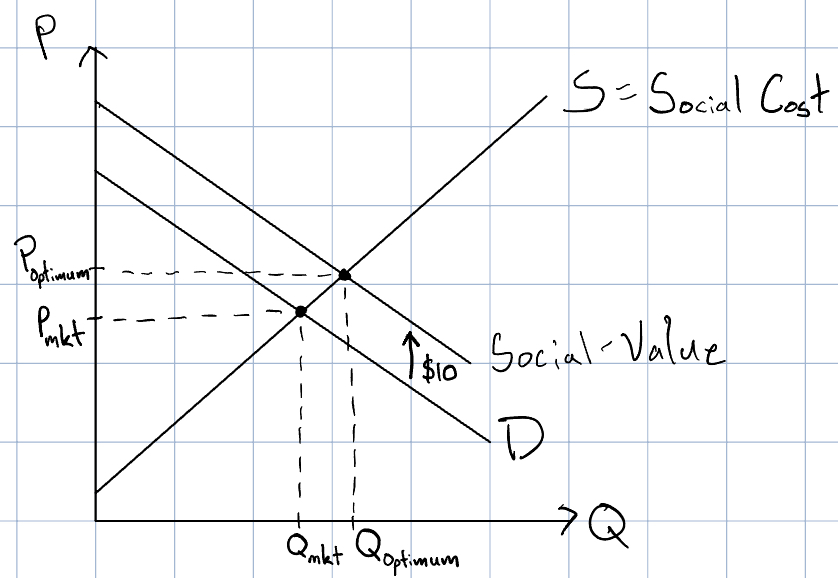
\includegraphics[width = 0.5\textwidth]{q2b}
		\end{center}
		
	\item Consumers of fire extinguishers have no incentive to account for the benefit of their fire extinguishers on their neighbors, so they under-consume relative to what is optimal. 
	
	\item The government could put a \$10 per unit subsidy on fire extinguisher consumption so that the private benefit of consumption matches the social benefit of consumption. 
	
	\end{enumerate}
	
\item

	\begin{enumerate}
	
	\item \phantom{x}
	
		\begin{center}
		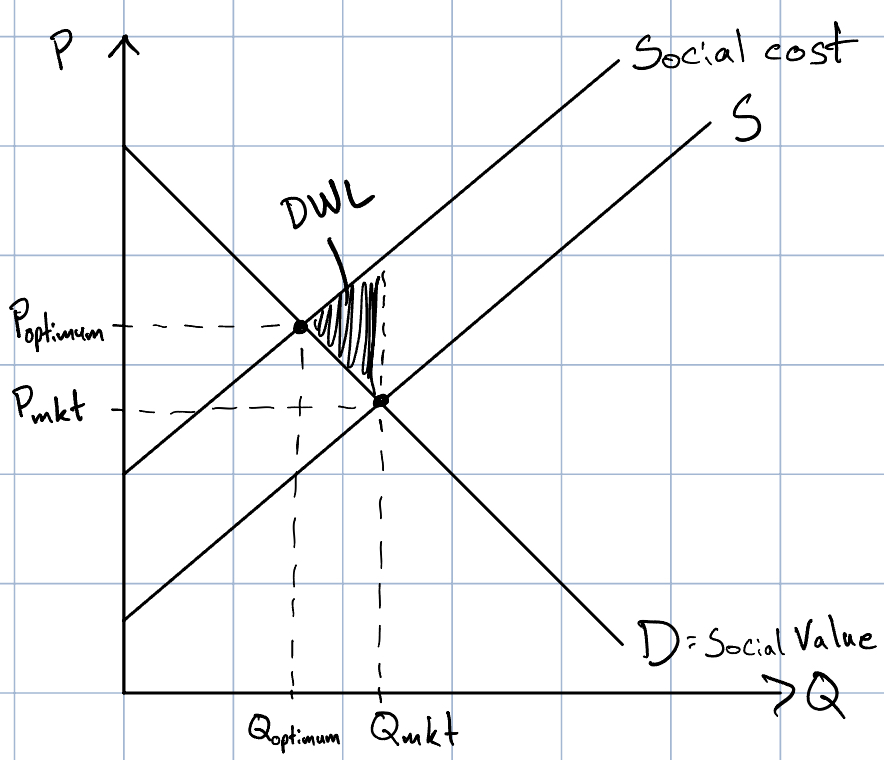
\includegraphics[width = 0.5\textwidth]{q3a}
		\end{center}
	
	\item After we surpass $Q_{Optimum}$, the social cost of alcohol exceeds the social value. The shaded region is the total difference between social cost and social value for all of the trades between $Q_{Optimum}$ and $Q_{mkt}$.
	
	\end{enumerate}

\end{enumerate}

\end{document}